\section{Evaluation}
\label{sec:evaluation}

The goal of our framework is to transform existing urban scenes into versions that: \emph{i)} people perceive more beautiful; \emph{ii)} contain urban elements typical of great urban spaces; \emph{iii)} are easy to interpret; and \emph{iv)} architects and urban planners find useful. To ascertain whether the framework meets that goal, next, we answer the following questions: 

\begin{description}
\item{\textbf{Q1}} Do individuals perceive our framework's scenes to actually be beautified?

\item{\textbf{Q2}}  Does our framework produce scenes that possess urban elements typical of great spaces?

\item{\textbf{Q3}}  Which urban elements are mostly associated with beautiful scenes?

\item{\textbf{Q4}}  Do architects and urban planners find our framework useful?

\end{description}


\subsection*{Q1 People's perceptions of beautified scenes}
To ascertain whether our framework's transformations are perceived by individuals as they are supposed to, we run a crowd-sourcing experiment on Amazon Mechanical Turk.  We randomly select 200 scenes, 100 beautiful and 100 ugly  based on whether they are at the bottom 10 and top 10 percentiles of the Trueskill's score distribution (Figure~\ref{fig:Trueskill}). Our framework then transforms each ugly scene into its beautified version, and each beautiful scene into its `uglified'. These scenes are arranged into pairs, each of which contains a beautiful scene and an ugly one. On  Mechanical Turk, we only select verified masters for our crowd-sourcing workers (those with an approval rate above 90\% during the past 30 days), pay them \$0.1 per  task,  and ask each of them to choose the beautiful scene in a pair.  We make sure to have at least 3 votes for each scene pair. Overall, our workers select the scenes that are actually beautiful 77.5\% of the times, suggesting that our framework's transformations are actually perceived by people to effectively be more beautiful. 


\subsection*{Q2 Are beautified scenes great urban spaces?}
To answer that question, we need to understand what makes a space great. After a careful review of the urban planning literature, we identify four factors~\cite{ewing2013measuring,alexander1977pattern} (summarized in Table~\ref{tab:Design_metrics}): great places mainly tend to be walkable, offer greenery, feel cozy, and be visually rich. 


\begin{table*}[h]
	\centering
	
	\resizebox{\linewidth}{!}{%
		\begin{tabular}{|c|p{14cm}|}
			\hline
			\textbf{Metric} & \textbf{Description}\\
			\hline
			Walkability  & Walkable streets are rated high on an aesthetic scale \cite{ewing2013measuring}. Walkable streets increase the social capital of a place and appeal to the exploring nature of human psyche. This implies that the urban space needs to address the fundamental need of people to walk and explore. This also implies that a walkable street must also be perceived as safe.\\
			\hline
			Green Spaces & Presence of Greenery is always pleasing to the eye. The literature always links urban beauty  to curated and well maintained green spaces, where social interactions can happen \cite{alexander1977pattern}. %, to be elements that bring a place 
			%together. 
			This 'social' aspect of greenery implies that dense forests or unkempt greens are not always related to the sense of beauty in urban scenes. \\
			\hline		
			Landmarks & Loosing a bearing in the city is not a very pleasant experience. Hence presence of recognisable and  guiding landmarks influences the perception of an urban space \cite{ewing2013measuring}.\\
			\hline
			Privacy-Openness &  A sense of privacy and a complimentary sense of openness are both influential in our perception of a place\cite{ewing2013measuring}. These values also tend to be related in an inverse 'U' fashion with beauty. \\ 
			\hline
			Visual Complexity & Visual complexity is a measure of how diverse a urban scene is. It manifests in terms of various design materials, textures and objects. Generally, visual complexity has an inverse 
			'U' relation with aesthetic values. The beauty and aesthetics of a place increases until it starts dropping because of 'too much' complexity\cite{ewing2013measuring}. \\
			\hline
	\end{tabular}}
	\caption{Urban Design Metrics}
	\label{tab:Design_metrics}
	%        \vspace{-5mm}
\end{table*}


To automatically extract visual cues related to these four factors, we select 500 ugly scenes and 500 beautiful ones at random, transform them into their opposite aesthetic qualities (i.e., ugly ones are beautified, and beautiful ones are `uglified'), and compare which urban elements related to the four factors distinguish uglified scenes from beautified ones. 

We extract labels from each of our 1,000 scenes using two computer vision algorithms. First, using PlacesNet~\cite{zhou2014learning}, we label our scenes according to a classification containing 205 labels (reflecting, for example, landmarks, natural elements), and retain the five labels with highest confidence scores for the scene. Second, using Segnet~\cite{badrinarayanan2015segnet}, we  label our scenes according to a classification containing 12 labels. Segnet is trained on dash-cam images, and the resulting lables are road, sky, trees,  buildings, poles, signage, pedestrians, vehicles, bicycles, pavement, fences, and road markings. 




\begin{figure}[h]
	\centering
	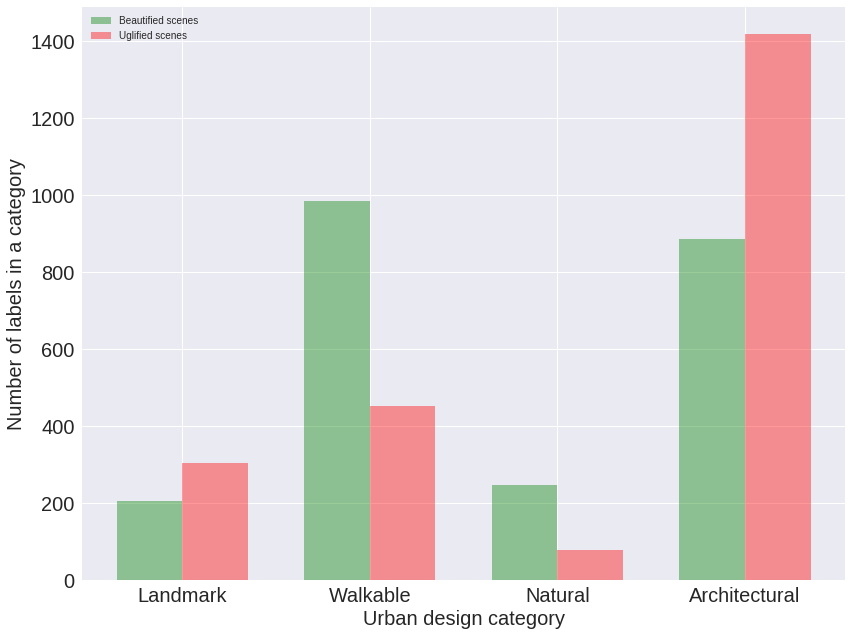
\includegraphics[width=\columnwidth]{Plot/taxonomyCount.png}
	\caption{Number of labels in specific urban design categories (on the $x$-axis) found in beautified scenes as opposed to those found in uglified scenes.}
	\label{fig:taxonomyCount}
\end{figure}


\begin{figure}[h]
	\centering
	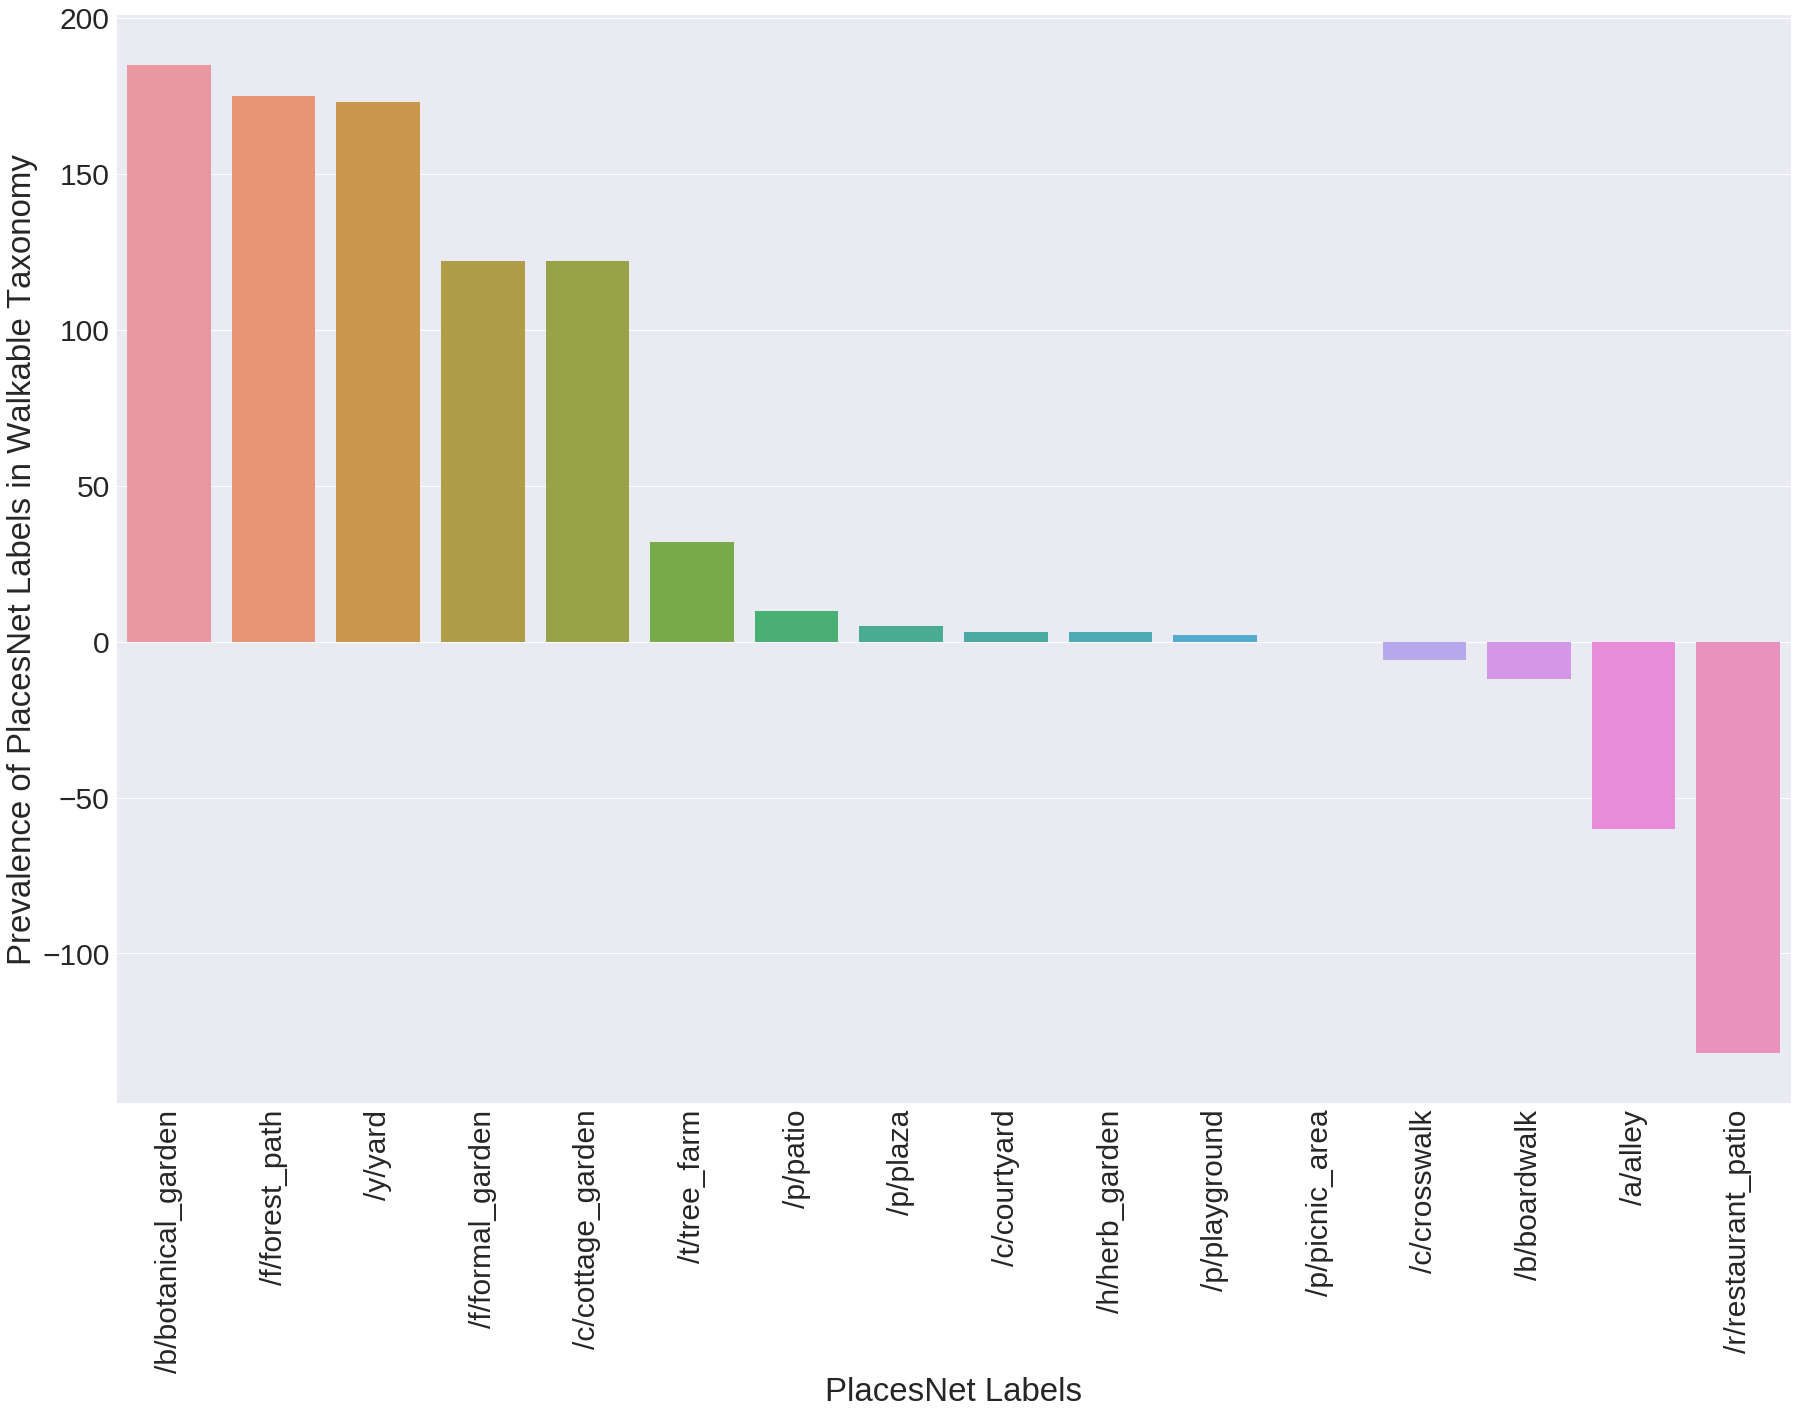
\includegraphics[width=\columnwidth]{Plot/walkable_taxonomy.png}
	\caption{Count of specific walkability-related labels  (on the $x$-axis) found in beautified scenes minus the count of the same labels found in uglified scenes.}
	\label{fig:WalkableTnomy}
\end{figure}


%**************************************************
\noindent
\emph{H1 Beautified scenes tend to be walkable.}
We manually select only the labels that are related to walkability. These labels include, for example, \textit{abbey , plaza , courtyard, garden, picnic area, park}. To test hypothesis \emph{H1}, we count the number of walkability-related labels found in beautified scenes as opposed to those found in uglified scenes (Figure~\ref{fig:taxonomyCount}): the former contain twice as much walkability labels that the latter. We then consider the prevalence of specific labels Figure~\ref{fig:WalkableTnomy}, and  find that beautified scenes tend to show gardens, yards, small path. By contrast, uglified ones tend to show built environment features such as shop fronts and broad sidewalks. 


\mbox{ } \\
%**************************************************
\noindent
\emph{H2 Beautified scenes tend to offer green spaces.}
We manually select only the PlacesNet's labels that are related to greenery. These labels include, for example, \textit{fields, pasture , forest, ocean, beach}. Then, in our 1,000 scenes, to test hypothesis \emph{H2}, we count the number of nature-related labels found in beautified scenes as opposed to those found in uglified scenes (Figure~\ref{fig:taxonomyCount}): the former contain more than twice as much nature-related labels that the latter.  To test this hypothesis further, we compute the fraction of `tree' pixels (one of SegNet's label) in beautified and uglified scenes. We find that beautification adds  32\% of greenery pixels, and uglification removes 17\% of greenery pixels. 


%We classify the 205 scene labels of PlacesNet into 4 categories, \textbf{L}andmarks , \textbf{A}rchitectural , \textbf{W}alkable , \textbf{N}atural. Each category is inspired from  urban design literature \cite{ewing2013measuring}.  Labels like \textit{Abbey , Plaza , Courtyard, Garden, Picnic Area, Park , etc} fall into the category of \textit{Walkable}, where as labels like \textit{Mansion, Castle, Dam , Airport, etc} fall in the category of \textit{Landmarks}. Labels like \textit{Residential neighborhood, Motel, hotel, restaurant, etc} fall in the category of \textit{Architectural} and labels like {fields, pasture , forest, ocean, beach etc } fall in the category \textit{Natural}. %All in all  For an image, we then measure its Wakability according to how many of the top-5 labels fall in category W. Similarly, we quantify presence of Greenery and Landmarks according to the frequency of N and L labels.%These higher-level LAWN labels represent  broader urban design motifs that constitute a liveable city we can detect through PlaceNEt. 


\begin{figure*}[!t]
	\centering
	\hspace*{-5mm}
	\subfloat[]{
		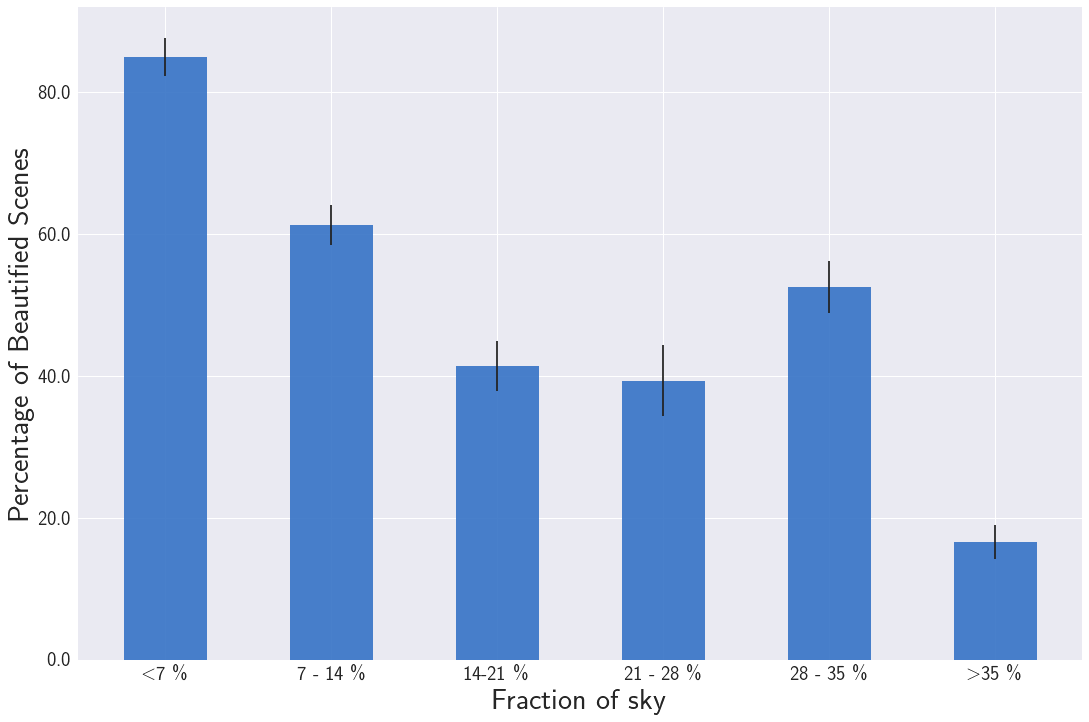
\includegraphics[width=0.45\textwidth, height = 5cm ]{Plot/BinnedPlot.png}
		\label{fig:skyBinned}
	}
	\subfloat[]{
		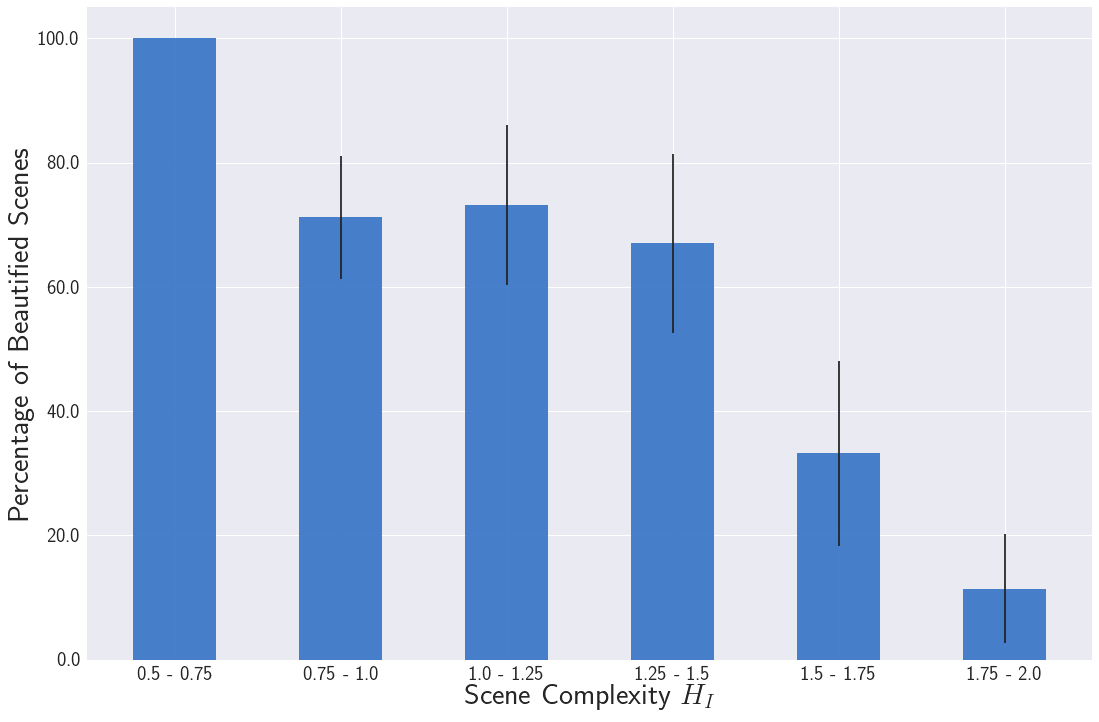
\includegraphics[width=0.45\linewidth, height = 5cm ]{Plot/binnedPlot_complexity.png}
		\label{fig:complexity}
	}
\vspace{-0.4cm}
\label{fig:bin_figures}
\caption{The percentage of scenes ($y$-axis): (a) having an increasing presence of sky (on the $x$-axis); and (b) having an increasing level of visual richness  (on the $x$-axis).}
\vspace{-0.4cm}
\end{figure*}



\mbox{ } \\
%**************************************************
\noindent
\emph{H3 Beautified scenes tend to feel private and `cozy'.}
To  test hypothesis \emph{H3}, we count the fraction of pixels that Segnet labeled  as `sky' and show the results in a bin plot in Figure~\ref{fig:skyBinned}:  the $x$-axis has six bins each of which represents a given range of sky fraction, and the $y$-axis shows the percentage of beautified \emph{vs.} uglified scenes that fall into the corresponding bin.  Beautified scenes tend to be cozier (lower sky presence) than the corresponding original scenes.


\mbox{ } \\
%**************************************************
\noindent
\emph{H4 Beautified scenes tend to be visually rich.}
To quantify to which extent scenes are visually rich, we measure their visual complexity~\cite{ewing2013measuring} as  the amount of disorder in terms of distribution of (Segnet) urban elements in the scene: 
\begin{equation}
H(X) = -\sum p(i)\log p(i)
\label{eq:entropy} 
\end{equation}
where $i$ is the $i^{th}$ Segnet's label. The total number of labels is twelve. The higher $H(X)$, the  higher the scene's entropy, that is, the higher the scene's complexity. To test hypothesis \emph{H4}, we show the percentage of scenes that fall into a given bin of complexity scores (Figure~\ref{fig:complexity}): beautified images tend have low to medium complexity, while uglified scenes are of high complexity.


%After detecting LAWN categories through PlacesNet labels,  we compute, for each image, the difference between the category frequency before and after transformation (e.g. how many 'Walkable' labels are added after beautification?). We then plot the aggregated difference-distributions for beautified and uglified image sets in Fig \ref{fig:taxonomyCount}.% Because the transformation is directly dependent on maximizing the classifier's certainty about an image being beautiful or ugly, this method directly gives us a  beautiful or ugly urban scene.
%This method provides insights regarding how transformations change the presence of scene types.


%From the literature, it is conjectured that privacy is great when one
%looks at personal spaces, but when it comes to public settings, there is an inverse 'U' relation with how private a place feels like. 
%Too much privacy discourages the fundamental human urge to explore a mystery. Too much openness  alerts the primal urge to feel safe. 
%\par
%\textit{[H3] Sense of Privacy has an inverse 'U' relationship with the sense of beauty }
%\par
%What \textit{H3} suggests is that sense of privacy is not always associated with beauty. 



%\begin{figure}[h]
%	\centering
%	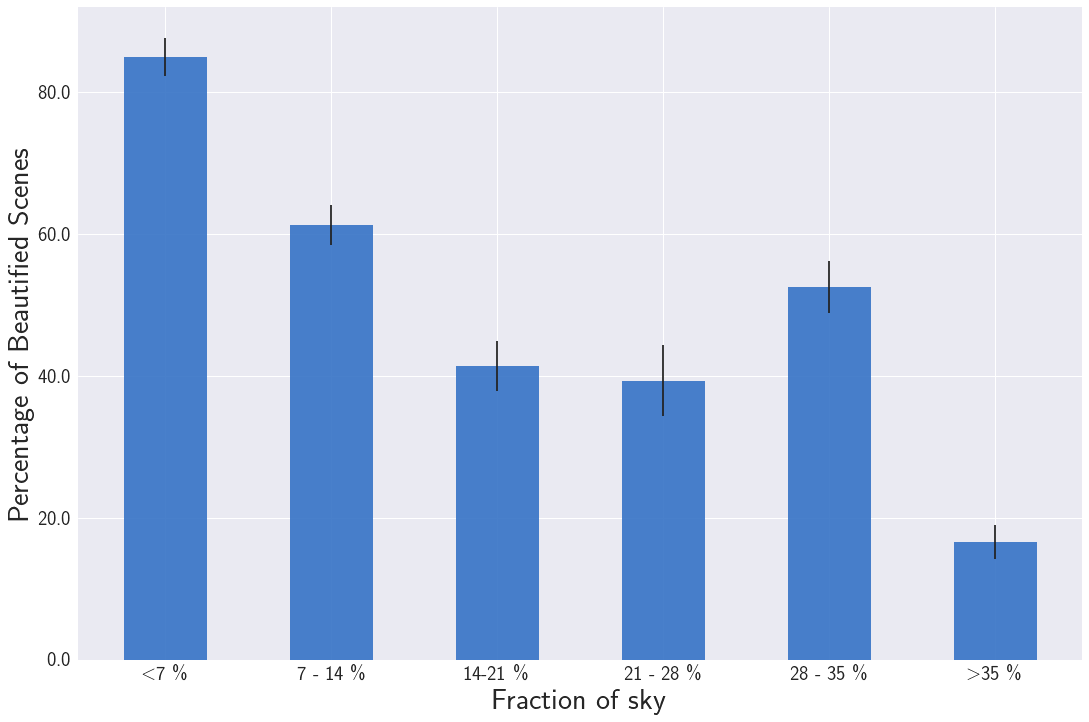
\includegraphics[width=\columnwidth]{Plot/BinnedPlot.png}
%	\caption{Binned Plot for Sky pixels across transformed images}
%	\label{fig:greenBinned}
%\end{figure}

%This effect can be individually seen from Fig \ref{fig:BuildingsCoverage} and Fig \ref{fig:TreeCoverage}. Beautification always prefers reduction of 
%visible buildings and increase in an overall green coverage \footnote{All distributions are tested using student-t tests and are found to have significantly hight T-statistic score (>>20) and p value << $10^{-5}$}. However this does not necessarily untangle the trade-off relationship of privacy-openness and beauty.

%To understand relation between openness and privacy, we repeat analysis as described in Section \ref{sec:vehicles}, for the amount of Sky and Tree pixels in a scene. The assumption here is these two objects in the scene are predominately driving the sense of openness. Adapting the Equation \ref{eq:regression} for the tree and sky pixel ratios we get different values for $\beta_1 , \beta_2 and \beta_3$. In this case the regression yields $\alpha = 0$ , $\beta_1 = 0.06$ , $\beta_2 = 0.10$ and $\beta_3 = -0.04$ . These values suggest that trees and sky, on their own have a positive impact on the beauty of a picture. 


%**************************************************
\subsection*{Q3 Urban elements of beautified scenes}

\begin{table}[t!]
	\centering
	\resizebox{\linewidth}{!}{%
	\begin{tabular}{|c|c|c|c|c|}
		\hline
		\textbf{Pair of urban elements} & \textbf{$\beta_1$}  & \textbf{$\beta_2$} & \textbf{$\beta_3$}  & Error Rate (Percentage)\\
		\hline
               \hline
		Buildings - Trees & -0.032 & 0.084  & 0.005  & 12.7 \\
		\hline
		Sky - Buildings & -0.08 & -0.11 & 0.064 & 14.4 \\
		\hline
		Roads - Vehicles  & -0.015  & -0.05 & 0.023  & 40.6 \\
		\hline
		Sky - Trees & 0.03 & 0.11 & -0.012 & 12.8  \\
		\hline
		Roads - Trees & 0.04  & 0.10 &  -0.031  & 13.5  \\
		\hline
		Roads - Buildings & -0.05  & -0.097  &  0.04  & 20.2  \\
		\hline
	\end{tabular}
	}
	\caption{Regression coefficients on a logistic run on a pair of predictors at the time.}
	\label{tab:regressioncoef}
    \vspace{-10mm}
\end{table}


To determine which urban elements are the best predictors of urban beauty and the extent to which they are so, we run a logistic regression, and, to ease interpretation, we do so on a pair of predictors at the time: 
\begin{equation}
Pr(beautiful) = logit^{-1}(\alpha + \beta_1 * V_1 + \beta_2 * V_2  + \beta_3 * V_{1}.V_{2} )
\label{eq:regression} 
\end{equation}
where $V1$ is the fraction of the scene's pixels marked with one Segnet's label, say, buildings (over the total number of pixels),  and $V2$ is the fraction of the scene's pixels marked with another label, say, trees. The result consists of three beta coefficients: $\beta_1$ reflects $V1$'s contribution in predicting beauty,  $\beta_2$ reflects $V2$'s contribution, and $\beta_3$ is the interaction effect, that, reflects the contribution of the dependency of $V1$ and $V2$ in predicting beauty. We run logistic regression on the five factors that have been found to be most predictive of urban beauty~\cite{quercia2014aesthetic, ewing2013measuring, alexander1977pattern}. 


Since we are using a logistic regression, the quantitative interpretation of the beta coefficients is eased by the ``divide by 4 rule''~\cite{vaughn2008data}: we can take $\beta$ coefficients and ``divide them by 4 to get an upper bound of the predictive difference corresponding to a unit difference'' in beauty~\cite{vaughn2008data}. For example, take the results in the first row of Table~\ref{tab:regressioncoef}. In the model $Pr(beautiful) = logit^{-1}(\alpha - 0.032 \cdot buildings + 0.084 \cdot trees + 0.005 \cdot  buildings \cdot trees)$, we can divide - 0.032/4 to get -0.008: a difference of 1 in the fraction of pixels being buildings corresponds to no more than a 0.8\% negative difference in the probability of the scene being beautiful. In a similar way, a difference of 1 in the fraction of pixels being trees corresponds to no more than a 0.021\% positive difference in the probability of the scene being beautiful. By considering the remaining results in Table~\ref{tab:regressioncoef}, we find that, across all pairwise comparisons, trees is the most positive element associated with beauty, while roads and buildings are the most negative elements. Since these results go in the direction one would expect, one might conclude that the scenes beautified by our framework are in line with previous literature, adding further external validity to our work. 




%**************************************************
\subsection*{Q4 Do architects and urban planners find it useful?}

\begin{figure*}[!t]
	\centering
	\hspace*{-5mm}
	\subfloat[]{
		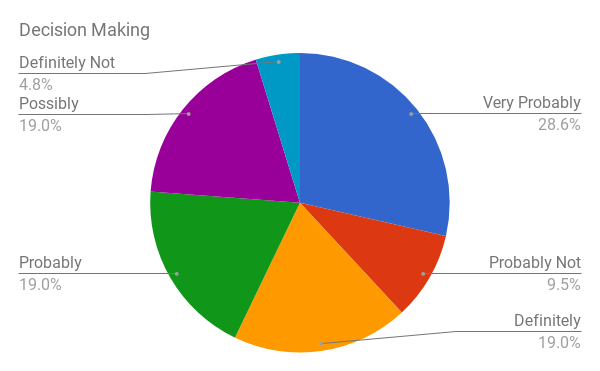
\includegraphics[width=0.3\textwidth ]{Plot/DecisionMaking.png}
		\label{fig:decision}
	}
	\subfloat[]{
		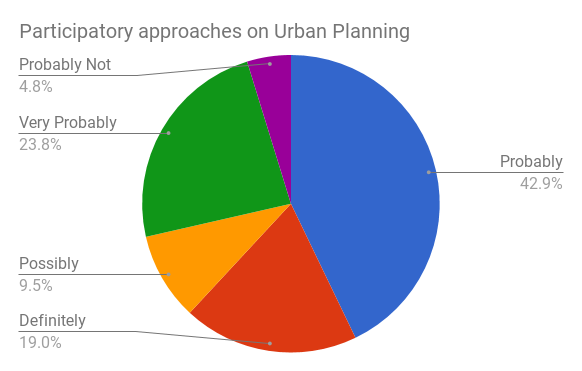
\includegraphics[width=0.3\linewidth ]{Plot/ParticipationUrbanPlanning.png}
		\label{fig:participation}
	}
	\subfloat[]{
		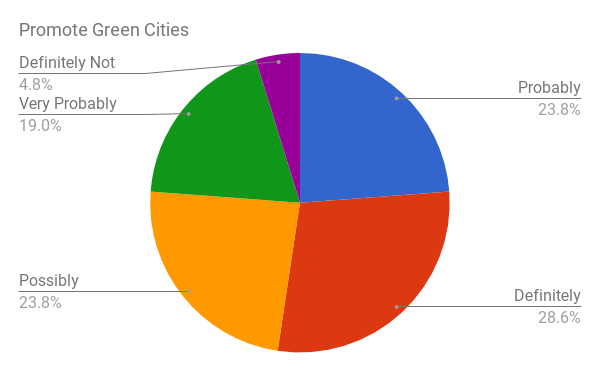
\includegraphics[width=0.3\linewidth ]{Plot/PromoteGreenCities.png}
		\label{fig:promotion}
	}
%	\vspace{-0.4cm}
	\caption{Urban expert polling on the extent to which an interactive map of ``FaceLifted'' scenes promotes: (a) decision making; (b) citizen participation in urban planning; and (c) promotion of green cities.}
	\label{fig:pies}
	\vspace{-0.4cm}
\end{figure*}

To ascertain whether practitioners find FaceLift potentially useful, we built an interactive map of the city of Boston in which, for  selected points, we showed pairs of urban scenes before/after beautification \textbf{[picture?]}. We then sent that map along with a survey to 20 experts around the world in the areas of architecture, urban planning, and data visualization.  The experts had to complete tasks in which they rated FaceLift based on how well it supports decision making, participatory urbanism, and promotion of green spaces among the general public. The results are show in Figure~\ref{fig:pies}: according to our experts, the tool can very probably supports decision making, probably support participatory urbanism, and definitely promote green spaces.  These results are  qualitatively supported by our experts' comments, which included: ``\textit{The maps reveal patterns that might not otherwise be apparent}'',  ``\textit{The tool helps focusing on parameters to identify beauty in the city while exploring it}'',  and ``\textit{The metrics are nice. It made me think more about beautiful places needing a combination of criteria, rather than a high score on one or two dimensions. It made me realize that these criteria are probably spatially correlated}''.






